\documentclass{standalone}

\usepackage{tikz}

\begin{document}
\Large
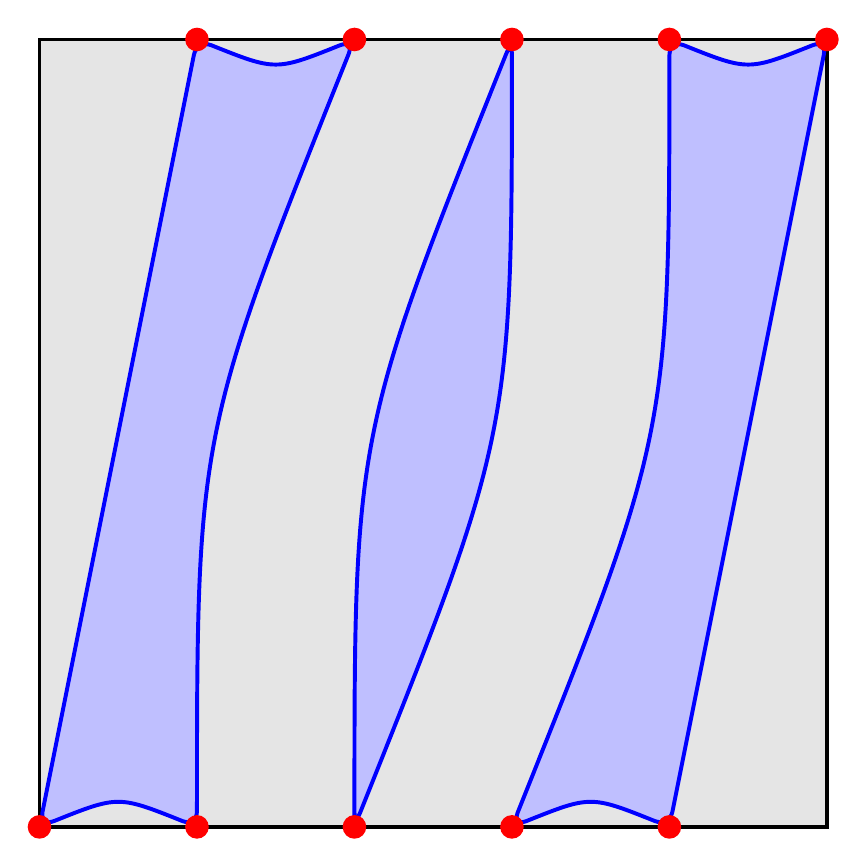
\begin{tikzpicture}
% \draw[help lines, black!30] (0,0) grid (25,12);
\draw[line width=0.5mm, black, fill=black!10] 
    (0,0) rectangle (10,10);
\draw[line width=0.5mm, blue, fill=blue!25, rounded corners=2mm] 
    (0,0) ..controls+(1,0.4).. 
    (2,0) ..controls+(0,5).. 
    (4,10) ..controls+(-1,-0.4).. 
    (2,10) -- cycle
    (4,0) ..controls+(2,5).. 
    (6,10) ..controls+(-2,-5).. cycle
    (10,10) ..controls+(-1,-0.4).. 
    (8,10) ..controls+(0,-5).. 
    (6,0) ..controls+(1,0.4).. 
    (8,0) -- cycle;
\fill[red] foreach \a in 
    {(0,0), (2,0), (4,0), (6,0), (8,0), 
     (2,10), (4,10), (6,10), (8,10), (10,10)}
    {\a circle (1.5mm)};
%\foreach \a/\b in 
%    {(0,0)/, (2,0)/1, (4,0)/2, (6,0)/3, (8,0)/4}
%    {\node[below=2mm] at \a {$A_{\b}$};};
%\foreach \a/\b in 
%    {(2,10)/1, (4,10)/2, (6,10)/3, (8,10)/4, (10,10)/}
%    {\node[above=2mm] at \a {$B_{\b}$};};
%\foreach \a/\b in 
%    {(1.5,5)/1, (5,5)/2, (8.5,5)/3}
%    {\node at \a {$\mathcal{C}_{\b}$};};
\end{tikzpicture}
\end{document}